\documentclass[12pt]{article}
\usepackage{ryblatex}

\setlength{\parskip}{0em}

\makeindex[
    name=terms,
    title={Term Index},
    columns=3,
    intoc=true
]

\makeindex[
    name=examples,
    title={Example Index},
    columns=2,
    intoc=true
]

\AddToHook{cmd/subsection*/after}{\addcontentsline{toc}{subsection}{#1}}

\usepackage{versions}
% \excludeversion{proof}

\title{DSC180A FA25: Rao-Yehudayoff Book Notes}
\author{Ciro, Darren, Ivy, Ryan}
\date{\today}

\begin{document}

\maketitle

\tableofcontents

\section{Deterministic Protocols}

Notes on Ch1 of the Rao-Yehudayoff book from the second meeting, Monday Oct 6 2025. Speakers: Ciro and Ivy. This chapter covers deterministic protocols; rectangles; richness; fooling sets. Basic lower bound methods.

\subsection{Rectangles}

A \term{deterministic protocol} is a pre-determined procedure between how patries commnicate for whatever problem we give it. The goal of this communication is to compute something deterministic based on the input. 

One way to model this is as a tree. Consider two parties, Alice and Bob. Alice has input $x$, Bob has $y$, and they wish to compute something based on $x,y$.

\begin{example}
[\ex{$\text{Eq}$} example] Suppose Alice and Bob work to find if $x = y$, equivalently compute
\begin{align*}
    \text{Eq}(x,y) = \begin{cases}
        1 & x = y, \\
        0 & x \neq y.
    \end{cases}
\end{align*}
Suppose further $x,y$ are two bits. We can represent this communication as a \term{tree}:
\begin{center}
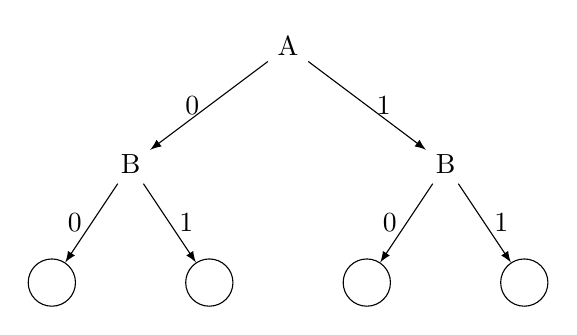
\begin{tikzpicture}[level distance=1.5cm,
%   every node/.style={circle,draw,minimum size=8mm,inner sep=0pt},
  edge from parent/.style={draw,-latex},
  level 1/.style={sibling distance=4cm},
  level 2/.style={sibling distance=2cm}
  ]
\node (A) {A}
  child {node (B1) {B}
    child {node[circle,draw,minimum size=6mm,inner sep=0pt,fill=white] {}
      edge from parent node[left] {0}
    }
    child {node[circle,draw,minimum size=6mm,inner sep=0pt,fill=white] {}
      edge from parent node[right] {1}
    }
    edge from parent node[left] {0}
  }
  child {node (B2) {B}
    child {node[circle,draw,minimum size=6mm,inner sep=0pt,fill=white] {}
      edge from parent node[left] {0}
    }
    child {node[circle,draw,minimum size=6mm,inner sep=0pt,fill=white] {}
      edge from parent node[right] {1}
    }
    edge from parent node[right] {1}
  };
\end{tikzpicture}
\end{center}
\end{example}

\begin{remark}
Notice that communication complexity presents a combinatorial setting to solve problems, which have much more mathematical tools compared to general complexity. Therefore, 
\end{remark}

\begin{lemma}
A protocol that sends $c$ bits has a protocol tree of depth $c$. This implies you can partition your matrix (whose rows are the possibilities of $x$ and columns $y$) into $2^c$ monochromatic rectangles. (Recall that a partition is a disjoint collection whose union is the whole thing.)
\end{lemma}

\begin{definition}
A \term{monochromatic rectangle} is a subset of the matrix $R \subseteq X \times Y$ such that if $(x,y), (x',y') \in R$, then $(x,y'),(x',y) \in R$. 
\end{definition}

\begin{example}
Consider the following matrix:
\begin{center}
    \begin{tabular}{c c}
        1 & 0 \\ 
        0 & 1
    \end{tabular}
\end{center}
This cannot be one monochromatic rectangle. However, 
\begin{center}
    \begin{tabular}{c c}
        1 & 1 \\ 
        1 & 1
    \end{tabular}
\end{center}
can be expressed as one monochromatic rectangle.
\end{example}

\begin{example}
Notice that the matrix for $\text{Eq}$ from Example \labelref{1.1} is just the identity matrix. By \labelref{1.4} there must be at least $n$ monochromatic rectangles, one for each $1$ on the diagonal. Therefore, no protocol exists that does better than $n$ bits communicated for $\text{Eq}$.
\end{example}

\begin{remark}
Notice that since we care about the worst case, that is all $x,y$, we care more about the number of rectangles, not the size of the rectangles; it is possible that our matrix is covered mostly by 1 rectangle, but many (hard) inputs can only be covered by very small rectangle.
\end{remark}

\subsection{Fooling Sets}

\begin{definition}
TODO; A \term{fooling set} is a subset $F \subseteq X \times Y$ such that if $(x,y), (x',y') \in F$ and $f: X \times Y \to {0,1}$ is the evaluation function, then either $f(x,y') \neq f(x,y)$ or $f(x',y) \neq f(x,y)$ such that it cannot be a single monochromatic rectangle.
\end{definition}

\subsection{Richness}

\begin{definition}
Define \term{richness} as a tuple $(u,v)$ describing the matrix of a protocol, particularly when $|X| < |Y|$ or vice versa. $u$ refers to the number of rows that have $v$ $1$s. Together with the size of $X,Y$, and the number of $1$s in the matrix, you can give an upper bound on the maximum size of a 1-monochromatic-rectangle and therefore a lower bound on the number of monochromatic rectangles (and thus communication complexity in general).
\end{definition}

\begin{example}
Consider the following matrix:
\begin{center}
    \begin{tabular}{c c c c}
        1 & 1 & 0 & 0 \\ 
        1 & 1 & 0 & 1 \\
        0 & 0 & 0 & 0 \\
        0 & 1 & 0 & 0
    \end{tabular}
\end{center}
The above has richness $(3,1), (2,2), (1,3)$. This tells us a maximum size of a 1-monochormatic rectangle (in particular, 2 by 2), which just happens to be tight here.
\end{example}

\begin{remark}
Note that rectangles and richness easily extend to relations, where there may be more than one possible input (for example, consider indexed sets $X$, $Y$ and finding $i$ where $X_i = Y_i$).
\end{remark}

\subsection{Computing Functions and Relations}

\begin{definition}
Define the \term{computational complexity} of $g: X \times Y \to \{0,1\}$ denoted $\CC(g)$ is the minimum depth of the protocol tree of $g$. Define $P(g)$ as the minimum number of leaves, equivalently, the number of monochromatic triangles of the protocol tree.
\end{definition}

\begin{lemma}
$P(g) \leq 2^{\CC(g)}$. Also, $\sqrt{\CC(g)} \leq \log_2 P(g) \leq \CC(g)$.
\end{lemma}

\begin{example}
Suppose $g : X \times Y \to \{0,1\}$ and $g$ requires $c$ bits of communication. Suppose we wish to compute $g^m$. If $g$ is a function, $\CC(g^m) = \CC(g)^m$ is an open problem. If $g$ is a relation, you cannot do this. TODO; See book why.
\end{example}

\begin{theorem}
$P(g^m) = P(g)^m$.
\end{theorem}

\begin{remark}
We can study the number of leaves but not the depth...
\end{remark}


\section{Lower Bounds for One-Way Communication: Disjointness, Index, and Gap-Hamming}

\begin{remark}
Recall that the one-way communication complexity for disjointness is $\Omega(n)$, even for randomized protocols.
\end{remark}

\begin{remark}
Recall that all constant error probabilities yield the same communication complexity, up to a constant factor. This is because the sucess of a protocol can be boosted though amplification via repeated trials.
\end{remark}

\begin{lemma}
Let $D$ be a distribution over the space of inputs $(x,y)$ to a protocol and $\epsilon \in (0,0.5)$ be its error. Suppose every deterministic one-way protocol $P$ with
\begin{align*}
    \Pr_D[P \text{ wrong on }(x,y)] \leq \epsilon
\end{align*}
has CC at least $k$. Then every randomized one-way protocol $R$ with two sided error at most $\epsilon$ on every input has communication cost at least $k$.
\end{lemma}

\begin{proof}
The idea is that we transfer randomness from the input into the protocol itself. Write $P$ as a distribution of deterministic protocols $P_1, \ldots, P_s$. Then on average the protocol is wrong at least epsilon times, completing the proof.
\end{proof}

\subsection{Index}

\begin{definition}
The index problem is where Alice has a list of $n$ bits and Bob has a $\log_2(n)$ bit index $i$ and they wish to compute the $i$th bit of Alice's input.
\end{definition}

\begin{theorem}
The randomized one-way communication complexity of index is $\Omega(n)$.
\end{theorem}

\begin{proof}
Let $D$ be the uniform distribution of inputs. We show every deterministic one-way protocol that uses $cn$ bits has error at least $1/8$, where $c$ is some small constant. By Lemma 2.3, this implies that every randomized protocol has error at least 1/8 on some input. \medbreak

Fix a deterministic protocol $P$ that uses $cn$ bits. There are $2^{cn}$ distinct messages that Alice sends. We show that
\begin{align*}
    \Pr[P \text{ is incorrect}] = \frac{d_H(x,a(z))}{n}
\end{align*}
where $d_H$ is the Hamming distance and $a(z)$ is Bob's guess; an \term{answer vector}. Think of each $a(z)$ as a ball of radius $n/4$ in the Hamming cube. Since there are only $2^{cn}$ balls of small radii, the union of all the balls is less than half of the Hamming cube. That is, there are at least $2^{n-1}$ bad inputs. \medbreak 

Fix some answer vector $a$. The number of inputs $x$ with hamming distance at most $n/4$ from $a$ is 
\begin{align*}
    1 + \binom{n}{1} + \binom{n}{2} + \binom{n}{n/4}
\end{align*}
where we choose how many bits to change from 0 (a itself) to $n/4$. Recall that
\begin{align*}
    \binom{n}{k} \leq \left(\frac{en}{k}\right)^k
\end{align*}
so the above is bounded by $2^{.861n} \leq 2^{n-1}$ for sufficiently large $n$.
\end{proof}

\subsection{Gap-Hamming}

\begin{remark}
Our current goal is to prove that every streaming algorithm that computes a $(1 \pm \epsilon)$ approximation of $F_0$ or $F_2$ needs $\Omega(\epsilon^{-2})$ space. We do this using reductions.
\end{remark}

\begin{definition}
Let $x,y$ be inputs interpreted as streams, i.e. vectors of numbers. Then the hamming distance $d_H(x,y) = 2F_0 - |x| - |y|$. So a one-way protocol that computer $F_0$ with CC $c$ yields a communiction protocol that computes $d_H$ with CC $c + \log_2 n$. Thus a $(1 \pm \nicefrac{1}{\sqrt{n}})$ approximation of $F_0$ yields a protocol that estimates $d_H$ up to $2 \sqrt{n}$ additive error with $\log_2 n$ extra communication.
\end{definition}

\begin{theorem}
The randomized one-way communication complexity of gap-hamming is $\Omega(n)$.
\end{theorem}

\begin{proof}
Consider an input to index, where Alice has $n$ bits and Bob $\log_2 n$ bits an index $i$. Suppose $n$ is odd and large. Alice and Bob can generate wihtout communicating, an input $(x',y')$ to gap-hamming using public randomness. 
\end{proof}
\section{Randomized Protocols}

\subsection{Defining Randomness}

\begin{definition}
To talk about randomness in communication protocols, we begin by giving a careful definition of it. A protocol uses \term{public randomness} or \term{public coins} when all parties have access to a common shared random string. We denote this string by $R$. \medbreak

A protocol uses \term{private randomness} or \term{private coins} if each party privately samples an independent random string. In the case of Alice and Bob, we call these strings $R_a$ and $R_b$ respectively. \medbreak

We require $R$, $R_a$, $R_b$, and the input $(X,Y)$ as independent uniform and the only source of randomness in the protocol. Thus, a random protocol is simply a distribution over deterministic protocols.
\end{definition}

\begin{lemma}
Every private coin protocol can be simulated by a public coin protocol.
\end{lemma}

\begin{proof}
Simply use the public coin as the private coin.
\end{proof}

\begin{lemma}
Every public coin protocol can be simulated by a private coin protocol, albeit with a small increase in the length of the protocol.
\end{lemma}

\begin{proof}
Deferred.
\end{proof}

\begin{definition}
By introducting randomness, we also allow \term{error} into our functions. There are two ways to measure the probability that a random protocol makes an error: \medbreak

A random protocol has error $\epsilon$ in the \term{worst-case error} if for every input, the probability that the protocol makes an error is at most $\epsilon$. That is, $\forall x,y$,
\begin{align*}
    \mathop{Pr}_{R,R_a,R_b} [\pi_{R,R_a,R_b}(x,y) \text{ is wrong}] \leq \epsilon,
\end{align*}
where $\pi_{R,R_a,R_b}$ is the deterministic protocol obtained by fixing said variables. \medbreak 

Given a distribution on inputs $\mu$, we say that a protocol has error $\epsilon$ with respect to $\mu$ if the probability that the protocol makes an error is at most $\epsilon$ when the inputs are sampled from $\mu$. That is,
\begin{align*}
    \mathop{Pr}_{R,R_a,R_b,(X,Y)} [\pi_{R,R_a,R_b}(X,Y) \text{ is wrong}] \leq \epsilon.
\end{align*}
The \term{length} of a protocol is defined to be the maximum depth of all the deterministic protocol tress the random protocol may generate.
\end{definition}

\begin{lemma}
If a randomized protocol never errors, then we can fix the randomness to obtain a deterministic protocol that is always correct.
\end{lemma}

\begin{corollary}
If a randomized protocol has less length than its deterministic counterparts, then it must introduce some form of error to the output of the protocol.
\end{corollary}

For any random protocal, we can convert it easily into a determanistic
protocal, simply by fixing a coin or input, and then consiter how it behaves.
Further, Public and Private coin protocals can be cycled between. When
converting from a private to a public protocal, we mearely need to had both
parties agree to share thier private coins. For public to private, it can be
shown that this conversion can be done with only an additional
$\log(\frac{n}{\epsilon^2}) + \mathcal{O}(1)$ bits.

\subsection{Yaos minimax Principle}

\begin{theorem}
Yao's Minimax principle is a very helpful principle for proving lowerbounds on
randomized protocals. Formaly, it is an extention of the general minimax
principle, $\min_{x\inA} \max_{y \in b} xMy = \max_{y \in B} \min_{x \in A}$,
to expectations over random variables. Informally, it states that the optimal
performance of any random protocal is equal to that of any determanistic
protocal who's input is sampled from a worst case distribution, chosen to be as
hard as possible for the algorithm to solve. Thus, for many random protocals,the process of finding a lower bound becomes that of finding such a worste case
input, and then proving the lower bound for that input.
\end{theorem}

\subsection{Equality}

In equality, Alice and Bob are given $n$ bit strings $x,y$ and wish to know if these strings are the same or not. We know its determinstic communciation complexity is $n+1$.

\begin{example}
\ex{Simple Random Equality Protocol:} Let Alice and Bob have a shared random coin of length $k2^n$. This allows Alice and Bob to recover a random function
\begin{align*}
    h : \{0,1\}^n \to \{0,1\}^k
\end{align*}
which we can treat as a hashmap. Then Alice can send $h(x)$ to Bob and Bob responds with a bit indicating if $h(x) = h(y)$. \medbreak

Here $k+1$ bits are communicated and the probability of making an error is at most $2^{-k}$; the probability $h(x) = h(y)$ yet $x \neq y$ is $2^{-k}$, the probability $k$ bits of $x,y$ are the same (when hashed).
\end{example}

\begin{remark}
Though the protocol is efficient it requires a large number of shared random bits. We can try to reduce the number of bits, introducing a new dimension to optimize in our protocols.
\end{remark}

\begin{example}
\ex{Error-correcting Equality Protocol} An (example of an) \term{error correcting code} is a function
\begin{align*}
    C : \{0,1\}^n \to [2k]^m
\end{align*}
such that if $x \neq y$, then $C(x)$ and $C(y)$ differ in all but $m/2^{-\Omega(k)}$ coordinates. (When $m = 10n$, for any $k$ most functions $C$ will be error-correcting codes.) \medbreak

Given a code, Alice can pick a random coordinate of $C(x)$ and send it to Bob, and Bob can check whether $C(x) = C(y)$. Alice takes $\log_2 m$ bits to send the index and $\log_2 2^k = k$ bits to send the value. Thus the protocol takes $O(\log n + k)$ bits of communication. \medbreak 

The probability of making an error is at most $2^{-\Omega(k)}$, by the definition of the error-correcting code.
\end{example}

\begin{example}
\ex{Greater-than Random Protocol} Deterministic protocols take $\log n$ bits. A randomized protocol taking $O(\log \log n)$ bits exists. \medbreak
A simpler random protocol in $O(\log \log n \cdot \log \log \log n)$ can be done by using the above equality protocol to check if the first $n/2$ most significant bits of $x,y$ are the same. This allows us to perform a binary search on which bit differs first.
\end{example}

\subsection{Disjointness}

\begin{example}
\ex{$k$-Disjoint Random Protocol} Suppose Alice and Bob are given sets $X,Y \subseteq [n]$, each of size at most $k$. They wish to check for intersection. By the rank method, at least $\log \binom{n}{k}$ bits are required. \medbreak

When $k \ll n$, the deterministic protocol of length $O(k)$ is more efficient than any deterministic protocol. Here is how it goes: \medbreak

Shared randomness is used to generate $R_1, R_2, \ldots \subseteq [n]$. Alice announces the smallest index $i$ with $X \subseteq R_i$ and Bob does the symmetry with $j$. This takes $2(\log i + \log j + 2)$ bits. Alice replaces her set with $X \cap R_j$ and Bob with $Y \cap R_i$. Notice that if $X \cap Y = \emptyset$ this remains true, and same if $X \cap Y \neq \emptyset$. \medbreak

Repeat the above until $O(k)$ bits are communicated. If either set becomes empty, $X,Y$ are disjoint. If both sets are non-empty, they conclude $X,Y$ intersect.
\end{example}

\begin{theorem}
In the above, Alice and Bob arrive at the correct conclusion with probability at least $2/3$.
\end{theorem}

\begin{lemma}
The expected length of the first step is at most $2(|X| + |Y| + 2)$.
\end{lemma}

\begin{proof}
The probability $R_1$ contains $|X|$ is $2^{-|X|}$. If it does not, then
\begin{align*}
    \E[i] = 2^{-|X|} \cdot 1 + (1 - 2^{-|X|}) (\E[i] + 1)
    \implies \E[i] = 2^{|X|}.
\end{align*}
Same for $Y$. Then
\begin{align*}
    \E[2 \log i + 2 \log j + 4] 
    \leq 2(\log\E[i] + \log\E[j] + 2)
    = 2(|X| + |Y| + 2).
    \tag*\qedhere
\end{align*}
\end{proof}

\begin{lemma}
In the second round, the expectation is that the sets are half as large. Formally, for $i \in [n]$ let $X_{i,s}$ be the indicator variable for if $i \in X$ before step $s$ on the above process. Define $Y_{i,s}$ similarly. If $X,Y$ are disjoint,
\begin{align*}
    \E \left[ \sum_{i \in [n]} \sum_{s=1}^\infty X_{i,s} + Y_{i,s} \right] \leq 4k.
\end{align*}
\end{lemma}

\begin{proof}
Notice
\begin{align*}
    \E \left[ \sum_{i \in [n]} \sum_{s=1}^\infty X_{i,s} + Y_{i,s} \right]
    = \sum_{i \in [n]} \sum_{s=1}^\infty \E[X_{i,s}] + \E[Y_{i,s}]. 
\end{align*}
If $X_{i,1} = 0$, then $X_{i,s} = 0$ for all $s$. If $X_{i,1} = 1$, the probability $X_{i,s} = 1$ is $2^{-s+1}$ so 
\begin{align*}
    \sum_{i \in X} \sum_{s=1}^\infty \E[X_{i,s}]
    = \sum_{i \in X} \sum_{s=1}^\infty 2^{-s + 1}
    \leq 2k.
\end{align*}
Applying the same to $Y_{i,s}$ gives $\leq 4k$.
\end{proof}

\begin{theorem}[Markov's Inequality]
For any random variable $X \geq 0$,
\begin{align*}
    \P(X \geq a) \leq \frac{\E[X]}{a}.
\end{align*}
\end{theorem}

\begin{lemma}
The previous lemma implies that the parties communicate at most $16k$ bits. By the Markov inequality, the probability the protocol communicates more than $3 \cdot 16k = 48k$ bits is at most $1/3$.
\end{lemma}

\subsection{Hamming Distance}

\begin{definition}
If Alice and Bob are given two strings $x,y \in \{\pm1\}^n$, define the \term{Hamming distance} as
\begin{align*}
    H(x,y) = \Delta(x,y) = |{i \in [n] \mid x_i \neq y_i}| 
    = \frac{n - \langle x,y \rangle}{2}.
\end{align*}
\end{definition}

\begin{definition}
Say that a protocol $\pi$ approximates $\Delta$ up to $m$ if
\begin{align*}
    |\pi(x,y) - \Delta(x,y)| \leq m
\end{align*}
for all inputs $x,y$. For $alpha < 1/2$, approximating $\Delta$ up to $\alpha n$ requires deterministic CC $\Omega(n)$.
\end{definition}

\begin{theorem}
\ex{Hamming Distance Random Protocol} Suppose Alice and Bob wish to estimate $\Delta$ up to $m$. Both use shared randomness to sample $i_1, \ldots, i_k \in [n]$ independently and uniformly. They communicate $2k$ bits the \term{empirical distance}
\begin{align*}
    \gamma = (1/k) \cdot |{j \in [k] \mid x_{i_j} \neq y_{i_j}}|
\end{align*}
and output $\gamma n$. 
\end{theorem}

\begin{lemma}
The probability of making an error is at most $1/e$. 
\end{lemma}

\begin{proof}
Deferred.
\end{proof}
\section{Number on Foreheads}

\subsection{Multi-Party Communication}

\begin{definition}
In \term{nunber on forehead} problems, we have $k$ parties where each party can see the input of all other parties but not themselves.
\end{definition}

\begin{remark}
Why study this weird setup? Normally we consider number in hand setups, where each party only knows their own number. The reason is that many of these tools are used to prove lower bounds. (Opposed to algorithms which focus more on lower bounds). Because number of foreheads is a much more powerful model than number in hand, we can show lower bounds for many more problems that do not even look like communciation. \medbreak

In particular, this model is applicable even when we allow shared information, but number in hand would not.
\end{remark}

\begin{example}
Consider the \ex{pointer chasing problem}. There are three players. The first player holds a pointer in $\log n$ bits to $n$ nodes. The second holds a permutation of the $n$ nodes. The third has labels for for the $n$ permuted nodes. If we have the number in hand model, this would take $2 \log n$ bits. However, with number for forehead, a trivial protocol takes $O(n)$ bits and a non-trivial one takes $O(n / \log n)$ bits.
\end{example}

\begin{example}
Consider \ex{equality with $k$ players}. Then you only need $k-1$ bits of communication. Consider the case with 3 players. Alice can see if Bob's number if equal to Charlie and send a $1$ if so. Bob can then do the same with Alice and Charlie.
\end{example}

\begin{example}
Consider the \ex{intersection with $k$ parties problem}, and each party has a set $X_i \subseteq [n]$ as input on their forehead. The goal is to compute
\begin{align*}
    |X_1 \cap X_2 \cap \cdots \cap X_k|
\end{align*}
We can map this as a matrix problem: Consisder a $k \times n$ matrix where entry $(i,j)$ means player $i$ has number $j$. Thus we want to count the number of columns with all $1$s, such as the middle column of the following matrix $k \times n$ matrix:
\begin{align*}
    \begin{bmatrix}
        1 & \cdots & 1 & \cdots & 0 \\ 
        \vdots & \ddots & 1 & \ddots & \vdots \\
        \vdots & \ddots & 1 & \ddots & \vdots \\
        \vdots & \ddots & 1 & \ddots & \vdots \\
        0 & \cdots & 1 & \cdots & 1
    \end{bmatrix}
    \in \F_2^{k \times n}.
\end{align*}
A simple $O(n)$ algorithm would have one player count all the other parties' numbers, then have another party verify it out. A more clever algorithm is below. \medbreak

For each party $i$, count $C_{i0}$, $C_{i1}$, and so on, where $C_{ij}$ is the number of columns containing exatcly $j$ ones visible to the $i$th party. The parties announce $C_{i,j}$ for all $i,j$. Thus the communciation complexity is at most $O(k^2 \log n)$.
\end{example}

The above example only works if given all $C_{ij}$ for all $i,j$, there is a unique possible count for the number of all $1$s columns. We show that now.

\begin{proof}
Let $Z_r$ denote the number of column with $r$ ones. We show there is a unique tuple $Z = (Z_0, \ldots, Z_k)$ consistent with the $C_{ij}$s. 

\begin{lemma}
Suppose $Z = A$, $Z = B$ are two solutions that are both consistent with all $C_{ij}$s. Then 
\begin{align*}
    |A_r - B_r| = \binom{k}{r} |A_0 - B_0|
\end{align*}
for each $r \in \{0,1,\ldots,k\}$.
\end{lemma}
\end{proof}

\begin{example}
Consider exactly 3 parties. Each party has a number from $[n]$ on their forehead, and they want to know if these sum to $n$. The trivial protocol takes $O(\log n)$ by announcing one number and having the party whose number was announced compute the sum. \medbreak

There is another protocol that takes $O(\sqrt{\log n})$. Take $\Delta = A + B + C - n$. One does $-A + 2(n - A - C)$. Another does $(n - B - C) + 2B$. \medbreak

\begin{theorem}
\term{Berhend's Coloring}: One can color the set $[m]$ with $2^{O(\sqrt{\log m})}$ colors with no monochromatic 3-term arithmetic progression. Namely, for each $a,b \in [m]$, if all three numbers $a, a+b, a+2b$ are in $[m]$, they do not have the same color.
\end{theorem}

Just by comparing the colors, they will know whether $\Delta = 0$ which is equivalent to knowing if the sum is equal to $n$.
\end{example}

\begin{remark}
Recent results have allowed us to show we need $2^{(\log m)^c}$ where $0 \leq c \leq 1$ is a small constant. The paper is very technical.
\end{remark}

\subsection{Cylinders}

\begin{definition}
Any set $S \subseteq X_1 \times \cdots \times X_k$ can be described by its \term{characteristic function}
\begin{align*}
    F_S(x_1, \ldots, x_k) = \begin{cases}
        1 & (x_1, \ldots, x_k) \in S \\
        0 & \text{otherwise}
    \end{cases}
\end{align*}
\end{definition}

\begin{definition}
A \term{cylinder} is a set constant in a dimension $X_s$.
\end{definition}

\begin{remark}
Let us take a step back. In the 2 player case, the inputs where the output is $1$ form $2^c$ rectangles. Cylinders are the greater than 2 dimension counterpart. Consider a decision tree with three players:
\end{remark}

\[\begin{tikzcd}
	&& {f(B,C)} \\
	& {g(A,C)} && \cdots \\
	\ldots && {f(B,C)} \\
	& {h(A,B)} && \ldots \\
	& {\text{Result}}
	\arrow["0"', from=1-3, to=2-2]
	\arrow["1", from=1-3, to=2-4]
	\arrow["0"', from=2-2, to=3-1]
	\arrow["1", from=2-2, to=3-3]
	\arrow[from=3-3, to=4-2]
	\arrow[from=3-3, to=4-4]
	\arrow[from=4-2, to=5-2]
\end{tikzcd}\]

Then the intersection forms at most $2^c$ cylinder intersections where the output is $1$.

\begin{remark}
TODO: Ramsey theory
\end{remark}

\newpage
\printindex[terms]

\newpage
\printindex[examples]

\end{document}